
\label{sec:Versuchsaufbau}
Der prinzipielle Aufbau einer Wärmepumpe ist in Abbildung \ref{fig:bild1} dargestellt und soll nun näher erläutert werden.

\begin{figure}
  \centering
  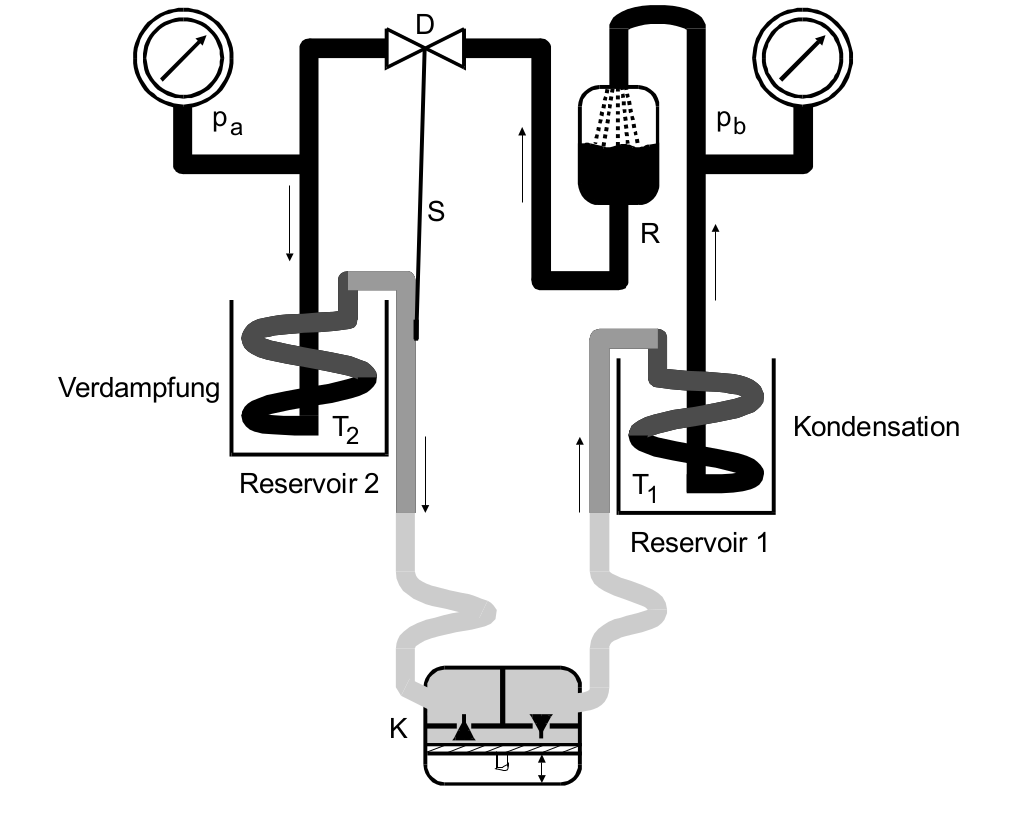
\includegraphics[width=0.85\textwidth]{content/aufbau_waermepumpe.png}
  \caption{Prinzipieller Aufbau einer Wärmepumpe \cite{Anleitung}}
  \label{fig:bild1}
\end{figure}

Bei einer Wärmepumpe wird Wärme von einem kälteren auf ein wärmeres Reservoir unter Aufwendung mechanischer Arbeit übertragen.

Um die Wärmeübertragung zu realisieren, verwendet man als Transportmedium ein reales Gas. Dieses verdampft bei geringerer Temperatur, nimmt dabei Wärme auf und kondensiert nachdem es komprimiert wurde, sodass Wärme an ein anderes Reservoir abgegeben wird.
Folglich sollte das verwendete Transportmedium eine möglichst große Kondensationswärme haben, damit möglichst viel Wärme pro Zeit übertragen werden kann.

Die Wärmepumpe ist so konzipiert, dass das verwendete Transportmedium bei der Temperatur $T_2$ und dem Druck $p_a$ gasförmig und auf der Seite des wärmeaufnehmenden Reservoir $R_1$ bei der Temperatur $T_1$ und dem druck $p_b$ flüssig ist.

Für die Wärmeerzeugung wird nun dem Reservoir $R_2$ Wärme entzogen, indem das Transportmedium kondensiert. Die Wärme wird also als Phasenumwandlungsenergie gespeichert.
Das somit entstandene Gas wird im Kompressor adiabatisch komprimiert und dabei stark erwärmt.
Das Gas strömt nun in das Reservoir $R_1$, kondensiert hier und gibt dabei die als Phasenumwandlungsenergie gespeicherte Wärme wieder ab.

Das nun wieder flüssige Transportmedium fließt nun durch einen Reiniger $R$, welcher verbliebene Gasblasen aus dem Transportmedium trennt.
Das Transportmedium erreicht nun das Drosselventil $D$.

Dieser wird reguliert von einem Steuermodul $S$. Das Steuermodul reguliert basierend auf der Temperaturdifferenz zwischen Ein-und Ausgang des Reservoir $R_2$ das Drosselventil so, dass maximal die Menge des Transportmediums $R_2$ zugeführt wird, welche auch verdampft wird, sodass keine Flüssigkeit in den Kompressor gelangt.
Am Drosselventil $D$ findet eine Entspannung, also ein Druckabfall des Transportmediums statt und der Prozess beginnt mit dem Kondensieren in $R_2$ erneut.
